
%=========================================================================================
\BiChapter{基于图表示学习与排序的文本情感溯源方法}{}



在这一章节将充分介绍我们提出的一种名为 Dag-Rank 的一步方法。它对文档中的子句对候选项进行排名,以提取情感原因对。总体架构如图\ref{fig:general}所示,由三个组件组成。第一个组件学习给定文档中子句的向量表示。第二个组件通过一个有向无环图模拟子句之间的关系,以获得更好的子句表示。第三个组件学习增强了相对位置建模的子句对表示,并对子句对候选项进行排名,以提取情感原因对。

\begin{figure}[ht]
    \vspace{20pt}
	\centering
    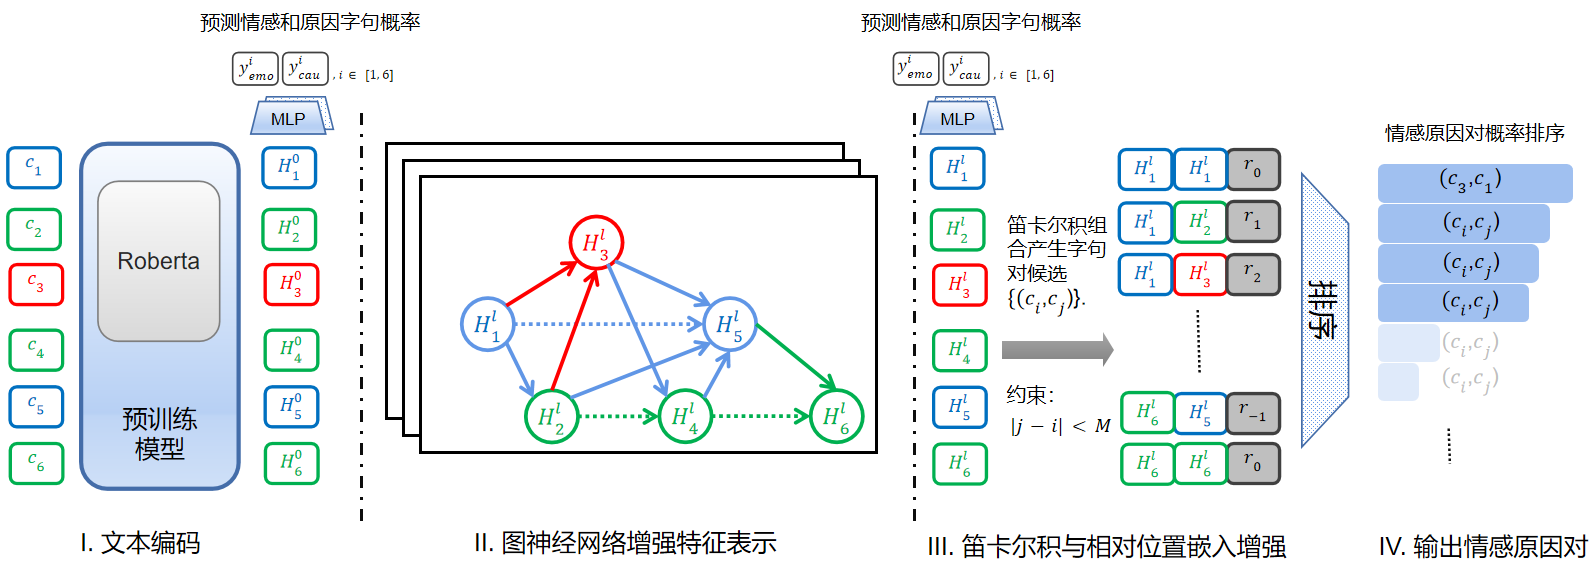
\includegraphics[width=1.02\linewidth]{figures/arch.png}
    \vspace{8pt}
	\caption{Dag-Rank总体架构:首先通过预训练模型获得给定文档中子句的向量表示,之后通过一个有向无环图神经网络模拟学习子句之间的关系,再通过相对位置建模增强的子句对表对子句对候选项进行排名,得到所需的情感原因对。}
    \label{fig:general}
    \vspace{7pt}
\end{figure}

    
\BiSection  {问题定义}{}

在本研究中,我们主要关注如何从一篇文档中提取情感-原因对。具体来说,给定一个文档 $D=(c_{1},c_{2},\dots,c_{|D|})$,在这里,$|D|$ 表示子句的数量,而第 $i$ 个子句 $c_{i}=(\omega^{i}{1},\omega^{i}{2},\dots,\omega^{i}_{|c_{i}|})$ 是一个单词序列。文档包含一个或多个情绪,每个情绪对应至少一个原因。我们的目标是在文档 $D$中提取所有的情绪-原因:
\vspace{3pt}  \begin{equation}
  P=\left\{\dots,(c_{i}^{e},c_{j}^{c})^k,\dots \right\},
  \label{eqn1}
\end{equation} \vspace{4pt}
其中$(c_{i}^{e},c_{j}^{c})^k$是$D$的第$k$个情绪原因对,$c_{i}^{e}$是包含某种情绪的情绪子句,而$c_{j}^{e}$是对应的原因子句。这两个子句构成一个情绪-原因对$(c_{i}^{e},c_{j}^{c})$。


% %=========================================================================================

    



\BiSection{文本编码}{文本编码}
\label{sec:encode}

在Dag-Rank方法中,我们首先对每个文本话语进行编码。每个话语被视为一个图节点,其特征可以由预训练的基于 Transformer 的语言模型提取。通常,我们会首先在每个数据集上对预训练语言模型进行微调,然后在训练时冻结其参数。这些预训练模型在大规模的文本数据上进行了自监督学习,能够学习到丰富的语义和语法信息。通过使用预训练语言模型,我们可以从每个文本话语中提取出高维度的特征表示,这些表示可以捕捉到文本的重要语义和上下文信息。在本次研究中,我们选择使用 RoBERTa-Base 作为特征提取器,这种基于Transformer的编码方法已经在自然语言处理领域证明了其有效性,并在多个任务上取得了优秀的性能\upcite{BERT}。具体地说,对于每个子句 $c_i=(w_{i1}, w_{i2},...,w_{in_i})$,我们在其标记前添加一个特殊标记 $[CLS]$,使输入形式为 ${[CLS],w_{i1}, w_{i2},...,w_{in}}$。然后,我们使用 $[CLS]$ 在最后一层的聚合嵌入作为 $c_i$ 的特征表示,用$\mathbf{c}_i$来表示。

\BiSection{有向图模型的图神经网络}{sec:builddag}

预训练模型主要专注于学习文本的线性结构,即将文本视为一个单词序列,并未能充分考虑文本中存在的复杂依赖和关系\upcite{luo2022biogpt}。
当文本数据具有图结构或者其中的元素之间存在某种非线性关系时,我们可以使用图神经网络(Graph Neural Network,GNN)与预训练模型结合来提供更多上下文信息,
在对话系统、知识图谱、社交网络或文档结构化等应用中,文本信息往往可以被建模为图形结构,这时,图神经网络就可以发挥其优势,有效地处理和学习这种复杂关系。
在我们的ECPE任务中,对话文本数据往往包含丰富的结构信息,如句子的句法结构、对话的回应结构等。利用图神经网络,我们可以明确地对这些结构信息进行建模,以提高模型对这些信息的理解。这对于很多自然语言处理任务(如情感分析、问答系统等)是非常有帮助的。

我们将文本中的话语视为图的节点,利用图神经网络来模拟话语间的关系,利用图的结构对节点之间的信息进行传播和更新,这样可以使得每个节点都能获取到它在图中邻居节点的信息。这种信息传播机制使得在图结构数据中的全局信息和局部信息都能被有效地捕获和利用。这种方法允许模型在捕获Roberta所提供的局部上下文信息的同时,也能处理和学习话语间的复杂关系。

\BiSubsection{有向图模型}{sec:builddag}
\label{sec:build_dag}

本研究设计使用一个有向无环图(Directed Acyclic Graphs, DAG)来模拟对话中的信息传播。 DAG由$\mathcal{G}=(\mathcal{V},\mathcal{E},\mathcal{R})$表示。在本文中,DAG中的节点是对话中的话语,即$\mathcal{V}=\{c_1,c_2,...,c_N\}$,边$(i,j,r_{ij})\in\mathcal{E}$表示信息从$c_i$传播到$c_j$,其中$r_{ij}\in\mathcal{R}$是边的关系类型。边的关系类型集合$\mathcal{R}=\{0,1\}$包含两种关系类型:$1$表示两个相连的话语由同一说话人说出,$0$表示否则。

在DAG中,首先决定何时一个话语会向另一个话语传播的三个约束进行了规定,即何时两个话语在DAG中连接:

\noindent
\textbf{方向性:}$\forall j>i, (j,i,r_{ji})\notin\mathcal{E}$。先前的话语可以向未来的话语传递信息,但未来的话语不能向后传递信息。

\noindent
\textbf{远程信息:}$\exists \tau< i, p(c_\tau)=p(c_i), (\tau,i,r_{\tau i})\in\mathcal{E}$,且$\forall j<\tau,(j,i,r_{ji})\notin\mathcal{E}$。对于除第一个话语$c_1$之外的每个话语$c_i$,存在一个先前的话语$c_\tau$,由与$c_i$相同的说话人说出。在$c_\tau$之前生成的信息称为远程信息,相对较不重要。我们假设当说话人说出$c_\tau$时,她/他已经意识到了$c_\tau$之前的远程信息。这意味着,$c_\tau$已经包含了远程信息,并将负责将远程信息传播到$c_i$。

\noindent
\textbf{局部信息:}$\forall l, \tau<l<i, (l,i,r_{li})\in\mathcal{E}$。通常,局部上下文的信息很重要。考虑第二个约束中定义的$c_\tau$和$c_i$。我们假设在$c_\tau$和$c_i$之间的每个话语$c_l$都包含局部信息,并且它们将局部信息传播到$c_i$。

第一个约束确保了对话是DAG,第二和第三个约束表明$c_\tau$是远程和局部信息的截止点。我们将$c_\tau$视为$p(c_i)$说出的第$\omega$个最新话语,其中$\omega$是超参数。然后,对于$c_\tau$和$c_i$之间的每个话语$c_l$,我们从$c_l$指向$c_i$建立一个有向边。我们在算法\ref{algo:build_DAG}中展示了构建DAG的上述过程。


\begin{algorithm}[t]

\begin{algorithmic}[1]
		\REQUIRE 对话 $\{c_1, c_2, ..., c_N\}$, 说话者身份 $p(\cdot)$, 超参数 $\omega$
		\ENSURE $\mathcal{G} = (\mathcal{V},\mathcal{E},\mathcal{R})$
		\STATE $\mathcal{V} \gets \{c_1, c_2, ..., c_N\}$ 
		\STATE $\mathcal{E} \gets \emptyset$
		\STATE $\mathcal{R} \gets \{0,1\}$ 
		\FORALL{$i \in \{2,3,...,N\}$}
		\STATE $c \gets 0$
		\STATE $\tau \gets i-1$
		\WHILE{$\tau > 0$ 且 $c < \omega$}
		\IF{$p(c_\tau) = p(c_i)$}
		\STATE $\mathcal{E} \gets \mathcal{E}\cup\{(\tau,i,1)\}$
		\STATE $c \gets c +1$
		\ELSE
		\STATE $\mathcal{E} \gets \mathcal{E}\cup\{(\tau,i,0)\}$
		\ENDIF
		\STATE $\tau \gets \tau-1$
		\ENDWHILE
		\ENDFOR
		\STATE 返回 $\mathcal{G} = (\mathcal{V},\mathcal{E},\mathcal{R})$
	\end{algorithmic}
\vspace{6mm}
\caption{从对话中构建DAG的基本算法}
\label{algo:build_DAG}

\end{algorithm}

\begin{figure}[h]
	\centering
    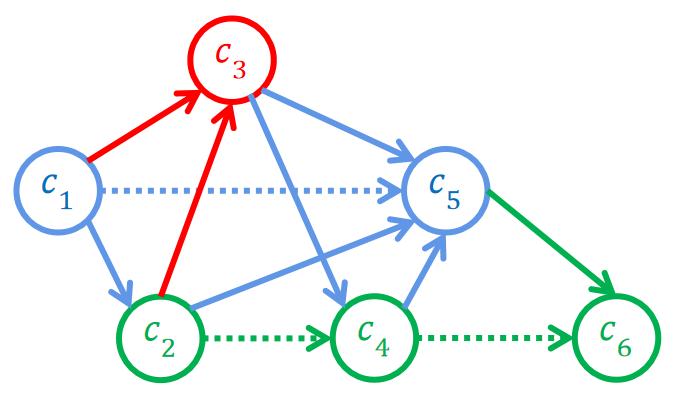
\includegraphics[width=0.5\linewidth]{figures/dag.png}
        \vspace{8pt}
	\caption{一个描述3个对话者中6句话语被建模为DAG的例子,图中实线为不同对话者的直接后继,虚线为同一个对话人的上一个话语。}
    \label{fig:dag}
    \vspace{10pt}
\end{figure}


图\ref{fig:dag}是我们建模DAG的一个实例,该例中为 DailyDialog 数据集中的一个片段,包含3个对话人的6句话语。总的来说,我们引入时间顺序和方向性:在传统的图神经网络(GNN)中,节点之间的信息交换通常是无序和无方向的。这种设计不适合处理具有明确时间顺序和方向性的对话数据。因此,我们引入了有向无环图(DAG)结构,让信息从过去流向未来,这符合对话的自然流程。与以前的工作\cite{ghosal2019dialoguegcn,ishiwatari2020relation}中开发的图结构相比,我们的DAG有两个主要优势:我们的DAG没有未来话语到先前话语的边,我们认为这更为合理和现实,因为查询话语的情感不应该在实践中受到未来话语的影响。其次,我们的DAG为每个话语寻找更有意义的$c_\tau$,而不仅仅是将每个话语与一定数量的周围话语连接起来。

我们对远程信息和局部信息进行区分:在对话中,对于当前话语的理解不仅依赖于其近邻(即前一句话语),也受到远程信息(例如前一段话语)的影响。我们的模型明确区分了这两种类型的信息,并且为每种类型的信息制定了不同的传播路径。这样可以更好地捕捉对话中的长距离依赖关系。
此外,该方法进一步考虑了话语的说话者:在对话中,同一说话者的连续话语往往具有更强的内在关联性,这是因为说话者的心理状态和意图在短时间内一般较为稳定。我们的模型通过连接同一说话者的连续话语,将这种关联性纳入到模型的设计中,从而更好地理解和预测对话的动态。

\BiSubsection{构建图神经网络}{}

本研究使用信息传递神经网络(Message Passing Neural Networks, MPNN)框架(如图\ref{fig:mpnn})来建模我们的工作。
我们描述操作在带有节点特征$x_v$和边特征$e_{vw}$的无向图$G$上的MPNN。
将此形式扩展到有向多重叠加的图神经网络比较简单。
在MPNN的前向传播中有两个阶段,一个信息传递阶段和一个读出阶段。信息传递阶段运行$T$个时间步,由信息函数$M_t$和顶点更新函数$U_t$定义。在信息传递阶段,基于消息$m_v^{t+1}$,图中每个节点的隐藏状态$h_v^{t}$会更新,公式如下:
\vspace{3pt}  \begin{equation} \label{eq:update}
\begin{aligned}
m_v^{t+1} & = \sum\limits_{w \in N(v)} M_t(h_v^t, h_w^t, e_{vw}) \\
h_v^{t+1} & = U_t( h_v^t, m_v^{t+1})
\end{aligned}
\end{equation} \vspace{4pt}
其中,在求和中,$N(v)$表示图$G$中$v$的邻居。读出阶段使用某种读出函数$R$计算整个图的特征向量,公式如下:
\vspace{3pt}  \begin{equation} \label{eq:output}
\hat{y} = R({h_v^T \mid v \in G }).
\end{equation} \vspace{3pt}

消息函数$M_t$、顶点更新函数$U_t$和读出函数$R$都是学习得到的可微函数。$R$作用于节点状态的集合,并且必须对节点状态的排列不变,以便MPNN对图同构不变。在接下来的部分,我们通过指定使用的消息函数$M_t$、顶点更新函数$U_t$和读出函数$R$来定义文献中的先前模型。注意,还可以通过引入图中所有边的隐藏状态$h_{e_{vw}}^t$并类似于等式\ref{eq:update}更新它们来在MPNN中学习边特征。

本研究使用的消息函数是 $M_t(h_v^t, h_w^t, e_{vw}) = A_{e_{vw}} h_w^t$,其中 $A_{e_{vw}}$ 是一个学习得到的矩阵,每个边标签 $e$ 都有一个(模型假定离散的边类型)。更新函数是 $U_t = \textrm{GRU}(h_v^t, m_v^{t+1})$。这项工作使用了权重绑定,因此在每个时间步 $t$ 都使用相同的更新函数。
\vspace{3pt}  \begin{equation} \label{eq:graph_level}
R = \sum\limits_{v \in V} \sigma \left( i(h_v^{(T)}, h_v^0) \right) \odot \left( j(h_v^{(T)}) \right),
\end{equation} \vspace{4pt}
其中,$i$ 和 $j$ 是神经网络,$\odot$ 表示元素间的乘法。


\begin{figure}[t]
	\centering
    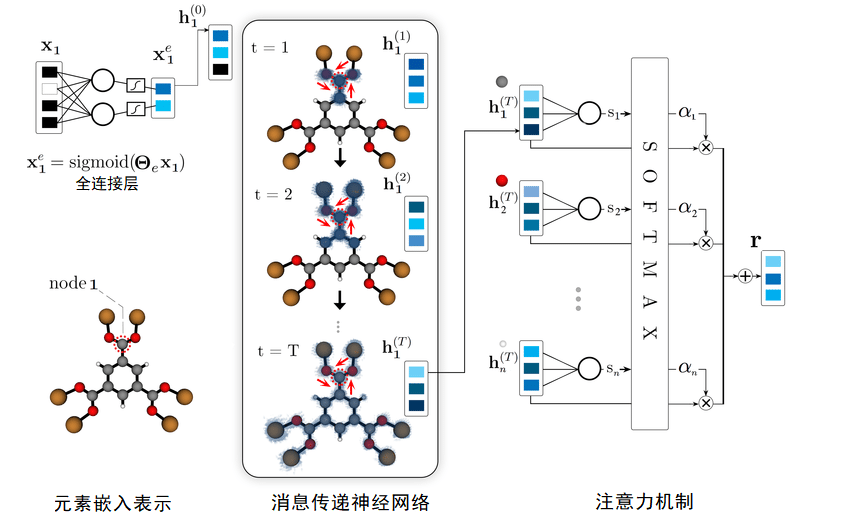
\includegraphics[width=0.95\linewidth]{figures/MPNN.png}
    \vspace{8pt}
	\caption{MPNN的框架是建立在消息传递神经网络(Message Passing Neural Network)的基础上的创新。与传统的模型不同,MPNN不是一个具体的模型,而是一种统一的表示方法,将现有模型的共性进行抽象和归纳。}
    \label{fig:mpnn}
\end{figure}


在MPNN的框架上,我们定义我们的图神经网络模型DAGNN,其工作方式类似于GNN和RNN的结合。它们按时间顺序为每个节点汇总信息,并允许所有节点从邻居那里收集信息并在同一层更新自己的状态:
\vspace{3pt}  \begin{equation}
H^l_i = f(\text{Aggregate}({H^{l}_j|j\in\mathcal{N}_i}),H^{l-1}_i).
\end{equation} \vspace{4pt}
我们将DAGNN用于提取文本特征的优点相当明显:通过允许信息在同一层内按时间顺序传播,DAGNN可以接触到远处的话语,并在整个对话中建模信息流,这对普通GNN来说几乎是不可能的。此外,DAGNN从几个相邻话语中收集信息,这听起来比RNN更有吸引力,因为后者只接收来自第 $(i\hspace{-0.07cm}-\hspace{-0.07cm}1)$ 个话语的信息。




我们在DAGNN的每一层 $l$ ,由于时间信息的流动,话语的隐藏状态应该从第一个话语到最后一个话语进行递归计算。
对于每个话语 $c_i$,通过使用 $c_i$ 在第 $(l-1)$ 层的隐藏状态来关注前继话语在 $l$ 层的隐藏状态,计算 $c_i$ 与其前继之间的注意力权重:
\vspace{3pt}  \begin{equation}
    \alpha^l_{ij} = \text{softmax}_{j\in\mathcal{N}_i}(W^l_\alpha[H^l_j\Vert H^{l-1}_i])
\end{equation} \vspace{4pt}
其中,$W_\alpha^l$ 是可训练参数,$\Vert$ 表示连接操作。

本研究应用了一种\emph{关系感知特征转换},以充分利用边的关系类型:
\vspace{3pt}  \begin{equation}
    M^l_i = \sum\limits_{j\in\mathcal{N}_i}\alpha_{ij}W_{r_{ij}}^lH^l_j,
\end{equation} \vspace{4pt}
其中,$W_{r_{ij}}^l\in\{W_0^l,W_1^l\}$ 是用于关系感知转换的可训练参数。这种关系感知特征转换的应用,可以使我们更好地利用图中的关系类型,提高模型对于情感溯源的准确性。

计算聚合信息 $M^l_i$ 后,我们使其与 $c_i$ 在上一层的隐藏状态 $H^{l-1}_i$ 交互,以获得当前层的 $c_i$ 的最终隐藏状态。在 DAGNN 中,通过让 $M^l_i$ 控制信息的传播,使用门控循环单元(GRU)来获得最终的隐藏状态:
\vspace{3pt}  \begin{equation}
\label{eq:DAGNN_H}
    \widetilde{H}^l_i = \text{GRU}^l_H(H^{l-1}_i, M^l_i),
\end{equation} \vspace{4pt}
其中,$H^{l-1}_i$、$M^l_i$ 和 $\widetilde{H}^l_i$ 分别是 GRU 的输入、隐藏状态和输出。

方程\ref{eq:DAGNN_H}中的过程称为\emph{节点信息单元},因为它专注于从过去的层传播到当前层的节点信息。节点信息单元可能适合 DAGNN 最初设计的任务。
然而,我们发现仅使用节点信息单元再当需要从上下文中推断出查询话语 $c_i$ 的情感时表现不佳,原因是在 DAGNN 中,上下文信息 $M^l_i$ 仅用于控制 $c_i$ 的隐藏状态的传播,而在这种情况下,上下文信息没有得到充分的利用。
因此,我们设计了另一个 GRU,称为\emph{上下文信息单元},来模拟历史上下文的信息流。在上下文信息单元中,GRU 中 $H^{i-1}_i$ 和 $M^l_i$ 的角色被颠倒,即 $H^{i-1}_i$ 控制 $M^l_i$ 的传播:
\vspace{3pt}  \begin{equation}
    C^l_i = \text{GRU}^l_M(M^{l}_i, H^{l-1}_i).
\end{equation} \vspace{3pt}
而$c_i$ 在第 $l$ 层的表示是 $\widetilde{H}^l_i$ 和 $C^l_i$ 的和:
\vspace{3pt}  \begin{equation}
    H^l_i = \widetilde{H}^l_i + C^l_i.
\end{equation} \vspace{3pt}

本研究使用的DAGNN模型结合了GNN和RNN的优点,加入了关系感知特征转换,设计了节点信息单元和上下文信息单元,这些创新使得我们的模型能有效加强提取文本特征,从而进一步提高处理和理解情感信息和情感原因的能力。

DAGNN模型第一层输入为\ref{sec:encode}章节介绍的子句表示,即$H^0_i=\mathbf{c}_i$。 通过堆叠$L$层DAGGNN层来对各个对话间关系建模,最后一层的输出是更新后的子句表示$H^L_i$。在后面的章节内,我们将用符号$H_i$作为子句$c_i$的加强后的特征表示,代表第$L$的最终输出$H^L_i$。
我们的图神经网络将预训练模型输出的子句特征$\mathbf{c}_i$做了进一步处理,考虑到对话文本中存在的复杂依赖和关系,捕捉了对话中的拓扑结构和节点之间的关系,提高了模型的理解能力。

为了预测一个子句是否是情感或因果子句,我们将子句 $c_i$更新前后的子句表示$H^0_i$和$H^l_i$输入到几个预输出层中。对于子句表示$H^0_i$,假设我们需要预测其是否为情感子句,相应预输出层是一个参数化为 $W^0_{emo}$ 和 $b^0_{emo}$ 的 MLP(多层感知器),它使用逻辑函数 $\sigma(.)$ 预测子句 $c_i$ 是情感子句的概率。这个概率被表示为 $\hat{y}_i^{emo}$,逻辑函数将 MLP 的输出映射到介于 0 和 1 之间的值,表示子句是情感子句的概率。而对于增强后的表示$H^l_i$,我们将使用另一个参数化为 $W^l_{emo}$ 和 $b^l_{emo}$ 的 MLP来进行预测。类似的,对于预测其是原因子句的概率$\hat{y}_i^{cau}$,我们用另外两个MLP对$H^0_i$和$H^l_i$分别进行预测,方法与上述相似。

\BiSection{使用基于核的相对位置嵌入对子句对进行排名}{Subequations}


排序模型的任务是将一组对象进行排序,使得排序结果与人类判断的排序结果尽可能相似。排序模型在实际应用中有着广泛的应用,例如在搜索引擎、推荐系统、广告排序、自然语言处理等领域。
在我们的研究中,我们需要对大量的子句对进行分类,这包括可能性高和可能性低的情感原因对。排序模型的引入,可以帮助模型更准确地预测子句对的情感原因关系的可能性,并将可能性较高的子句对排在可能性较低的前面,从而提高模型的预测精度和效率。表\ref{tab:pointrank}展示了机器学习分类回归任务中传统拟合方法和偏序排序方法的异同。


\begin{table}[h]
\vspace{15pt}
	\centering
	\renewcommand{\arraystretch}{1.2}
	\centering\wuhao
	\caption{常见提取问题中二分类方法和排序方法两种方法的特点和应用情况。}  \label{tab:pointrank} \vspace{4mm}
	\begin{tabularx}{\textwidth} { 
   >{\centering\arraybackslash}p{3cm} 
   >{\centering\arraybackslash}X 
   >{\centering\arraybackslash}X 
 }
	\toprule[1.5pt]
        处理方法   & 二分类     & 排序  \\ \midrule[1pt]
输入  & 特征 $x$     & 特征列表 $\textbf{x} = \{x_i\}_{i=1}^n$  \\ 
输出  & 二分类结果 $y=f(x)$   & 排序列表  $\text{sort}(\{f(x_i)\}_{i=1}^n)$  \\ 
损失  & MSE, BCE(二分类交叉熵)等 &
		\multicolumn{1}{>{\raggedright\arraybackslash}X}{
PRanking, Margin Ranking Loss等
		} 
\\ 
特点比较 &   
		\multicolumn{1}{>{\raggedright\arraybackslash}X}{
该方法简单直观,易于理解和实现,其输出每个样本的评分或偏好,这种评分可以更容易地理解和解释模型的结果。此外该方法适用于各种推荐场景,这种通用性使得该方法在实践中广泛使用。
		} 
      & 
		\multicolumn{1}{>{\raggedright\arraybackslash}X}{
该方法能够更好地捕捉到样本对之间的相互关系和排序信息,提供更准确的推荐结果。然而,它的训练过程相对较复杂,并且需要构造负样本,可能会增加训练的计算和存储开销。
		} 
\\
\bottomrule[1.5pt]
\end{tabularx}
 \vspace{10pt}
\end{table}


为了以端到端的方式提取情感原因对,我们的方法不仅需要学习子句对的表示,还需要根据这些表示对子句对进行排名,以确定最可能的情感原因对。在这个过程中,两个子句之间的相对位置是一个关键的指标。因此,我们通过引入相对位置嵌入,将这种相对位置信息融入到子句对表示的学习过程中。在许多自然语言处理(NLP)任务中,模型需要理解文本的顺序和上下文关系,这就涉及到位置编码或位置嵌入的问题。相对位置嵌入是一种常见的解决方案,它可以捕捉句子中词语的相对位置关系,从而帮助模型理解文本的语义和语境。


本研究基于的一个假设是,如果两个子句之间的相对位置过大,那么它们构成情感原因对的概率将会非常小。因此,给定文档$D=(c_{1},\ldots,c_{|D|})$,我们将两个子句的相对位置(绝对值)$|j {-} i|$ 小于或等于某个值 M 的每个子句对$ (c_i, c_j)$ 视为情感原因对的候选项。我们从文档 D 中构造一组子句对候选项:
\vspace{3pt}  \begin{equation}
\mathcal{P}'=\{(c_i,c_j)|-M\le j-i\le+M\} ,
\end{equation} \vspace{4pt}


对于每个子句对候选$p_{ij}=(c_i,c_j)\in\mathcal{P}'$,其初始化表示是通过连接三个向量获得的:子句$c_i$的表示$\boldsymbol{H}_i$、子句$c_j$的表示$\boldsymbol{H}_j$以及它们的相对位置$j-i$的嵌入$r_{j-i}$。我们使用一个单层MLP来学习其表示:
\vspace{3pt}  \begin{equation}
p_{ij}=\text{ReLU}(\boldsymbol{W}_p[\boldsymbol{H}_i;\boldsymbol{H}_j;\boldsymbol{r}_{j-i}]+\boldsymbol{b}_p),
\end{equation} \vspace{4pt}
其中$\boldsymbol{W}_p$和$\boldsymbol{b}_p$是可学习的参数。
传统方法对于每一个相对位置$m\in\{-M,...,-1,0,+1,...,M\}$通过从均匀分布中随机采样来初始化嵌入$r_m$。然后每个相对位置嵌入都将一同进行模型训练过程的学习。然而,传统的相对位置嵌入方法往往只考虑单一的相对位置,而忽略了不同相对位置之间可能存在的相互影响。这可能会限制模型的理解能力和预测性能。
我们希望建模不同相对位置之间的相互影响,以进一步改进相对位置嵌入。
为此,对于每个相对位置$m\in\{-M,...,M\}$,我们使用一个径向基函数(Radial Basis Function, RBF)作为核函数$K_m(\cdot)$来模拟$m$与其他相对位置之间的影响:
\vspace{3pt}  \begin{equation}
\mathsf{K}_m(j)=\exp\left(-\dfrac{(j-m)^2}{\sigma\kappa^2}\right),
\end{equation} \vspace{4pt}
其中$j\in\{-M,...,M\}$是可能的相对位置值之一,$\sigma$是核函数的宽度参数。这样,我们就可以通过考虑不同相对位置之间的相互影响来更好地表示相对位置嵌入。

我们选择使用RBF核函数来建模不同相对位置之间的影响,主要有两个原因。首先,RBF核函数能够捕捉相对位置之间的相似性,因为它的值随着两个位置的距离增大而减小。这符合我们的直觉,即相对位置接近的词语应该有更强的关联性。其次,RBF核函数的形式简单且易于计算,这有利于提高模型的训练效率。

然后,我们通过整合其他相对位置的影响来增强基本的嵌入$r_m$:
\vspace{3pt}  \begin{equation}
\boldsymbol{r}_m'=\sum\limits_{j=-M}^{+M}\mathsf{K}_m(j)\cdot\boldsymbol{r}_j.\quad(9),
\end{equation} \vspace{4pt}
其中,$\mathsf{K}_m(j)$是核函数$K_m(\cdot)$在$j$处的取值。其背后的直觉是,如果$j$接近$m$,$r_j$将对$\boldsymbol{r}_m$产生比其他远离$m$的相对位置更大的影响。图\ref{fig:kernel}展示了$m=-1$的情况。当$\sigma_K\rightarrow0$时,基于核函数的嵌入会退化为基础嵌入。因此,我们的基于核函数的嵌入方案可以被视为基础嵌入的正则化版本。


\begin{figure}[ht]
	\centering
    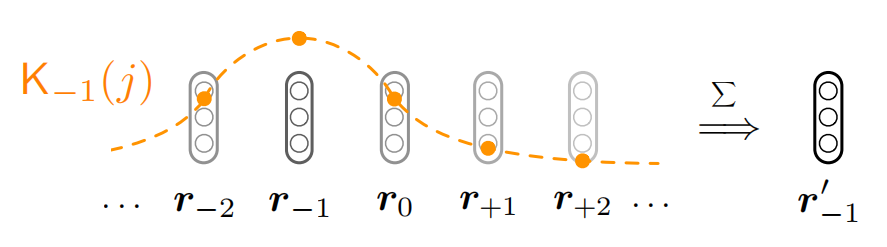
\includegraphics[width=0.7\linewidth]{figures/kernel.png}
	\caption{使用RBF核函数计算$r_{-1}$的例子。}
    \label{fig:kernel}
\end{figure}

这样,我们就可以考虑到不同相对位置之间的相互影响,进一步改进位置嵌入的表示能力。
我们接着采用带有激活函数$f_{\text{act}}(\cdot)$的排名层(由U和$b_r$参数化)来生成每个子句对候选的排名得分$\hat{y}_{ij}$。
\vspace{3pt}  \begin{equation}
    \hat{y}_{ij}=f_{\mathrm{act}}\left(\boldsymbol{w}_r^\top\boldsymbol{p}_{ij}+b_r\right),
\end{equation} \vspace{4pt}

我们将$\hat{y}_{ij}$表示每个子句对的排名得分。这是通过带有激活函的排名层生成,其作用是对每个情感原因对的重要性或相关性进行量化。在下一步提取中,我们将用其进行情感原因对提取。

% \BiSection{字典提取法}{Subequations}

% 在测试时,一个关键问题是如何根据所有候选情感原因对的排名分数提取潜在的情感原因对。需要注意的是,很难确定一个整体阈值分数,该分数可用于将候选项分成情感原因对和负面项。
% 我们采用基于词典的提取方案来从测试文档的前N个排名列表$\{p^1,p^2,...,p^N\}$中获取情感原因对。我们首先提取排名最高的情感原因对$p^1$(得分最高)。然后,对于每个剩余的子句对$p^i = (c^{i,1},c^{i,2})\in \{p^2,\ldots,p^N\}$,我们使用情感词典来确定子句$c_{i,1}$是否包含情感词。如果是,则将该子句对$p^i$提取为情感原因对。因此,我们的模型能够从给定的文档中提取多个情感原因对。

\BiSection{阈值提取法}{Subequations}

在测试时,一个关键问题是如何根据所有候选情感原因对的排名分数提取潜在的情感原因对。需要注意的是,很难确定一个整体阈值分数,该分数可用于将候选项分成情感原因对和负面项。
我们采用基于阈值的提取方案来从测试文档的前N个排名列表${p^1,p^2,...,p^N}$中获取情感原因对。我们将$f_{\mathrm{act}}$设置为\textit{sigmoid}函数以计算\textit{logistic} 概率,它能将模型的输出映射到0和1之间,从而直接被解释为概率。这种概率化的输出有助于我们理解模型的确定性,并为预测结果提供了置信度。此外,使用\textit{sigmoid}函数也允许我们设定一个阈值,根据这个阈值进行决策,使得模型的输出可以很自然地转换为类别预测。我们首先提取排名最高的情感原因对$p^1$(得分最高)。然后,对于每个剩余的子句对$p^i = (c^{i,1},c^{i,2})\in {p^2,\ldots,p^N}$,我们检查子句$c_{i,1}$是否出现在情感子句列表中。如果出现,则计算$p^i$的 \textit{logistic} 概率。如果该子句对作为情感原因对概率大于预定阈值,则将该子句对$p^i$提取为情感原因对。因此,我们的模型能够从给定的文档中提取多个情感原因对。


    
\BiSection{优化方法}{Subequations}
\label{sec:loss}
% 我们将 $c_i$ 在所有 DAG-ERC 层的隐藏状态的连接作为其最终表示,并通过前馈神经网络获得预测的情感:

% \begin{eqnarray}
% &&H_i = \parallel_{l=0}^{L} H^l_i,\\
% &&z_i = \text{ReLU}(W_HH_i+b_H),\\
% &&P_i = \text{Softmax}(W_zz_i+b_z),\\
% &&\widehat{y}_i = \text{Argmax}_{k\in\mathcal{S}}(P_i[k]).
% \end{eqnarray}

在许多机器学习和深度学习模型中,损失函数的设计是为了引导模型学习到我们希望它掌握的特定知识或者执行特定任务。
在我们的损失函数中,我们需要考虑几个部分。第一部分是度量子句对的排名分数。这是通过点对排序损失来完成的,排序损失的作用是通过比较两个对象之间的相对排序关系来训练模型。通过最小化排序损失,可以使得模型能够更准确地对一组对象进行排序,从而提高排序结果的质量。与其他损失函数相比,排序损失能够更直接地衡量模型对相对排序关系的预测能力,因此在排序问题中被广泛使用。我们对主损失函数定义如下:
\vspace{3pt}  \begin{equation}
\mathcal{L}_{\mathrm{pair}}=\sum_{\{p^{+},p^{-}\}\in\mathcal{P}_{p^{+} \succ p^{-}} }\operatorname*{max}\{0,-(y^{+}-y^{-})+\gamma \} ,
\end{equation} \vspace{4pt}
其中,$\gamma$是一个边界超参数,$p^+$和$p^-$是正样本和负样本子句对,它们的真实标签分别为1和0(因此$p^+$的得分$y^+$应该高于$p^-$的得分$y^-$),$\gamma$是一个边界超参数,用于控制正负样本之间的最小距离。这个损失函数的目的是将情感-原因对的分数分离出来,并将情感-原因对之间的分数差异最小化。排序损失也可以用于其他一些需要比较两个对象之间的相对关系的任务中。例如,如果我们想要训练一个模型来预测两个句子之间的相似度,我们可以将相似度定义为句子之间的相对排序关系,然后使用排序损失来训练模型。这种方法已经被成功应用于自然语言处理中的一些任务,例如文本匹配、问答系统等。

我们也可以使用传统的二分类交叉熵来计算损失,其作为典型的基于样本点的逐点方法(Pointwise) 关注的是绝对的预测分数。这种方法每次考虑一个输入样本,不考虑样本之间的相对排序关系,仅仅考虑预测样本的得分,有着更高的计算效率,其特性也与深度学习模型很适合。二分类损失函数如公式\ref{eq:binary}。
\vspace{3pt}  \begin{equation}
\label{eq:binary}
\mathcal{L}_{\mathrm{pair}}=\sum\limits_{p_{ij}\in\mathcal{P}'}-(y_{ij}\log\hat{y}_{ij}+(1-y_{ij})\log(1-\hat{y}_{ij})),
\end{equation} \vspace{4pt}
在这里,$y_{ij}\in\{0,1\}$是子句对$p_{ij}$的真实标签(如果$p_{ij}$是一个情感-原因对,则$y_{ij}=1$),$f_{act}(\cdot)$是激活函数。

第二部分的损失函数与子句的基本属性有关。我们考虑以下设置:首先,情感子句和原因子句在文本中是不同的,有着各自独特的语义和语境特征。在这个情况下,我们的主要目标是让模型能够准确地提取情感-原因对,但在实现这个主要目标的同时,我们也希望模型能够理解和区分情感子句和原因子句。如果我们只用一个损失函数去监督学习,那么模型可能无法准确区分这两种类型的子句,从而影响情感-原因对的准确提取。我们知道一个子句是否是情感/原因子句,因此我们使用两个交叉熵损失函数$\mathcal{L}_{\text{emo}}$和$\mathcal{L}_{\text{cau}}$来监督两个预输出预测。这两个损失函数的定义如下:
\vspace{3pt}  \begin{equation}
\mathcal{L}_{\text{emo}} = -\sum_{i=1}^{M}\sum_{t=1}^{N_i} y^{\text{emo}}_{i,t}  \text{log} \hat{y}^{\text{emo}}_{i,t},
\end{equation} \vspace{4pt}
其中,$M$ 是训练对话数量,$N_i$ 是第 $i$ 个对话中话语的数量,$y^{\text{emo}}_{i,t}$ 是实际标签,表示该字句是否为情感子句。  
\vspace{3pt}  \begin{equation}
\mathcal{L}_{\text{cau}} = -\sum_{i=1}^{M}\sum_{t=1}^{N_i} y^{\text{cau}}_{i,t}  \text{log} \hat{y}^{\text{cau}}_{i,t},
\end{equation} \vspace{4pt}
其中,$M$ 是训练对话数量,$N_i$ 是第 $i$ 个对话中话语的数量,$y^{\text{cau}}_{i,t}$ 是实际标签,表示该字句是否为情感子句。  
通过同时监督情感子句和原因子句的预测,我们为模型提供了更多的监督信息,使得模型能够从多个角度学习和理解数据。 


我们将上述两部分的总和作为文档$D$的最终损失函数$\mathcal{L}$:
% ,其中$\beta$是控制$\mathcal{L}_{\text{kl}}$比率的一个超参数:
\vspace{3pt}  \begin{equation}
    \mathcal{L} = \mathcal{L}_{\text{pair}} + (\mathcal{L}_{\text{emo}} + \mathcal{L}_{\text{cau}}),
    % + \beta \mathcal{L}_{\text{kl}}
\end{equation} \vspace{4pt}
这形成了对子句表示学习和子句对排名的两级监督。通过这种方式,我们的优化方法在损失函数中考虑了多个层面,以尽可能准确地提取出情感-原因对,并保证这些对的分布符合实际情况。在后续的实验中,我们将验证这种优化方法的有效性。


\BiSection{本章小结}{MethodConclusion}

我们提出了一种名为Dag-Rank的一步方法,用于文本情感原因对提取。
% 该方法的总体架构由三个组件组成。第一个组件学习给定文档中子句的向量表示。第二个组件利用有向无环图模拟子句之间的关系,以获得更好的子句表示。第三个组件学习增强了相对位置建模的子句对表示,并对子句对候选项进行排名,以提取情感原因对。
在Dag-Rank方法中,我们首先通过预训练模型获得给定文档中子句的向量表示,将文本转换成计算机方便理解计算的特征。我们设计了一个有向无环图(DAG)来模拟对话中的信息传播并建立 DAGGNN 图神经网络加强我们的子句特征。图中的节点是对话中的话语,边表示信息的传播关系。通过约束条件,我们确定了两个话语在DAG中连接的时机。这样的设计允许信息在同一层内按时间顺序传播,并允许节点从邻居节点那里收集信息并更新自己的状态。
另一个关键组件是基于核的相对位置嵌入,我们假设相对位置较大的子句对构成情感原因对的概率较小,它将相对位置信息融入到子句对表示的学习过程中,帮助模型理解文本的语义和语境。
最后,我们采用基于阈值的提取方案从排名列表中提取潜在的情感原因对。根据排名分数,我们逐步提取具有较高概率的子句对作为情感原因对。我们的优化方法包括排序损失函数、交叉熵损失函数和KL散度损失函数。排序损失函数用于准确预测情感原因对的相对排序关系,交叉熵损失函数帮助模型理解和区分情感子句和原因子句。
% KL散度损失函数用于约束它们的分布相似性。
通过这些损失函数的组合,我们在多个层面上优化模型,以提高情感-原因对的准确性和分布特征的学习。

我们的方法综合利用了子句表示学习、有向无环图模拟和相对位置建模等技术,以提取文本中的情感原因对。通过这种一步方法,我们能够更准确地捕捉情感原因对,并提高情感对提取的效果和效率。在后续的实验中,我们将验证这种优化方法的有效性。